\chapter{Methodology for Q-learning and Deep Q Network}
\label{Ch:methodology}

The main methodologies we are using for the research are Q-Learning and Deep Q Network(DQN). Here are some explanations about those methodologies.

\section{Q-learning}
Q-Learning is one of the Reinforcement Learning algorithms that attempts to learn the value of being in a given state, and taking a specific action there. Q-table is a table of values for every state(row) and action(column) possible in the environment. Within each cell of the table, we learn a value for how good it is to take a given action within a given state.  We start by initializing the table to be all zeros, and then as we observe the rewards we obtain by taking various actions, we update the table accordingly.

When updating the Q-table, Bellman equation is used. Bellman equation’s concept is that the expected long-term reward for a given action in a given state is equal to the immediate reward gained from the current action plus the expected reward from the best future action taken at the following state. Q-table is used to estimate the long-term reward. As shown below, Q-value for a given state(s) and action(a) should equal to the current reward(r) plus the maximum discounted($\lambda$) future reward expected according to Q-table for the next state$(s’)$ we would end up in. 
$$Q(s,a) = r + \lambda (\max (Q(s’,a’))$$

In Q-learning, for every training process, we first check whether the state already exists in the q-learning table, if it exists, we choose the action with the largest Q-value. If it doesn’t exist, we build a new empty line of this state and random choose action. Then we update the value in the q-learning table by  Q-TABLE learning formula .

As we use q-learning model, we need to discretize the states and actions. For actions, we discretize it by choosing actions as the weight of stock A of the total portfolio value and only keep one decimal. So we define the action vector as $(0, 0.1, 0.2, …, 0.9, 1)$. For the states, we tried two models. We first use the pair of stocks’ close price, but it is not general enough to be used as states in q-learning model. Then we generalize the states by using the pair of stocks’ close price change, and only keep two decimals. After that, we generalize our states by using another method. We using the slopes of the linear regression functions of the stocks’ each fixed period(3 days, 10 days).

For the reward function, at the first we simply used portfolio value change as a reward. However, as for portfolio management, we should not only consider the profit, but the risk. Thus we use sharpe ratio as the model’s reward function. Sharpe ratio formula 

\subsection{Q-learning Algorithm}
\def\skipl{0.2in}
\vspace{\skipl}
\fbox{
\begin{minipage}{5in}
Initialising $Q(s,a)$ arbitrarily 

Repeat (for each episode):

Initialise $s$

Repeat (for each step of a episode):

Choose $a$ from $s$ using policy derived from $Q$ (e.g. $\epsilon$ greedy)

Take action $a$, observe $r$, $s’$
\begin{equation}\label{eq:q-update}
Q(s,a) \leftarrow Q(s,a)+\alpha (r+\gamma \max_{a'} Q(s',a')-Q(s,a))
\end{equation}
\begin{equation}\label{eq:s-update}
 s \leftarrow s'
\end{equation}
Equation \eqref{eq:q-update} and \eqref{eq:s-update} are the update equations.
\end{minipage}}
\vspace{\skipl}

\section{Deep Q Network (DQN)}
Deep Q Network uses the techniques from deep learning to approximates Q-score, since in Q-Learning both state and action state need to be discrete and calculating and optimizing Q-score is both time and memory consuming. The key is that we apply the deep neural network to approximate the Q-function. We know that neural network is used to find out the right weights by the back propagation process so it can be used to map all state-action pairs to rewards. One standard example for neural network is using the convolutional neural network (CNN). 

Due to the problem of correlation between states and non-stationary targets, when we train the neural network, we store transition in memory M, and randomly sample mini-batch from M and replay to solve the problem. Plus, we separate the target network and copy the network regularly to solve non-stationary targets problem. Do a Forward Pass to get all possible Q values from the current state $s_t$.
\begin{enumerate}{}
\item Do a Forward Pass to get new state $s_{t+1}$ and argmax $a_{t+1}$. (Action that give us biggest Q-value)
\item Set Q-value target to $r+\gamma  \max Q(s',a')$ where $r$ is the reward and $\gamma$ is the discount rate.
\item Then use the backpropagation and stochastic gradient descent to update the network.
\end{enumerate}

Since CNN is a regression process, then the loss function will be squared.
$$L(\theta )=\frac{1}{2} \Big( R(s,a,a')+\gamma  \max Q(s',a';\theta)-Q(s,a;\theta) \Big)^2$$
\subsection{Algorithm}
\begin{figure}[H]
\begin{center}
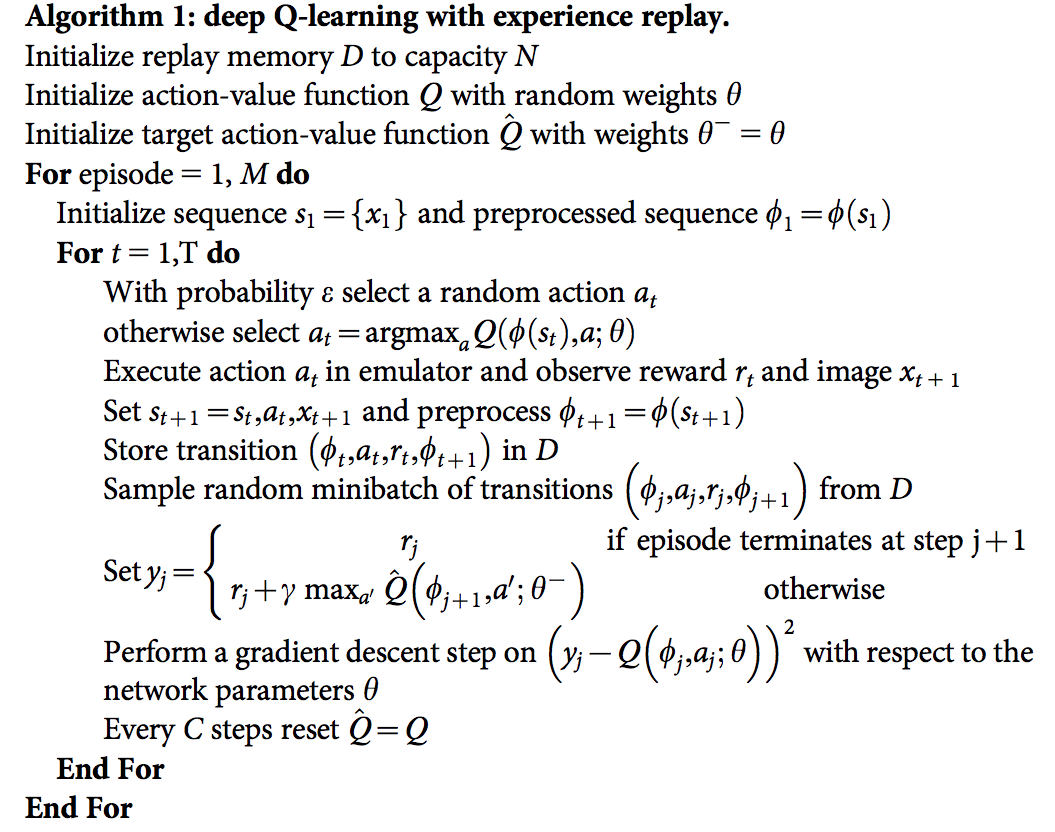
\includegraphics[clip, width=1\textwidth]{Graphics/DQN.png} \caption{Deep Q-Network algorithm}
\end{center}
\end{figure}